\documentclass[12pt,letterpaper]{article}
\usepackage[utf8]{inputenc}
\usepackage{geometry}
\geometry{margin=1in}
\usepackage{graphicx}
\graphicspath{{images/}}
\usepackage{tikz}
\usepackage{wrapfig,graphicx}
\usetikzlibrary{shapes.geometric, arrows}
\usepackage[most]{tcolorbox}
\renewcommand{\baselinestretch}{1.0}
\usepackage{multirow}
\usepackage{makecell}
\usepackage{natbib}
\usepackage{titlesec}
\bibliographystyle{plainnat}
\font\myfont=cmr12 at 20pt
\usepackage[font={scriptsize,it}]{caption}
\usepackage{titlesec}
\usepackage{setspace}

\renewcommand\theadalign{bc}
\renewcommand\theadfont{}
\renewcommand\theadgape{\Gape[4pt]}
\renewcommand\cellgape{\Gape[4pt]}
\titlespacing\subsection{0pt}{12pt plus 3pt minus 5pt}{0pt plus 2pt minus 1pt}

\title{\vspace{-2.5cm}\myfont From Narrative Text to VerbNet-Based DRSes}
\author{}
\date{\vspace{-5ex}}

%\tikzstyle{decision}=[diamond,draw,fill=blue!20,text width=4.5em,text badly centered,node distance=3cm,inner sep=0pt]  
\tikzstyle{io} = [trapezium, trapezium left angle=80, trapezium right angle=100, minimum width=1cm, minimum height=0.5cm, text width=5em, text badly centered, draw=black, fill=blue!15]
\tikzstyle{process1}=[rectangle,draw,fill=green!15,text width=6.5em,text badly centered,rounded corners,minimum height=2em]
\tikzstyle{process2}=[rectangle,draw,fill=orange!15,text width=6.5em,text badly centered,rounded corners,minimum height=2em] 
\tikzstyle{arrow}=[draw,-latex']  
%\tikzstyle{startstop}=[draw,ellipse,fill=red!20,node distance=3cm,minimum height=2.5em]  

\begin{document}
	
	\maketitle
	\subsection*{\small Introduction}
	\noindent Computational linguists have long studied various logic forms for capturing essential semantic information carried by narratives. Among these, discourse representation structure (DRS) \citep{kampreyle93} form is designed to acquire the entities, entities’ property, events, event types, the occurring time of events, and event arguments. In this paper, we describe a system called Text2DRS that takes English narrative as an input and outputs a DRS in Neo-Davidsonian style. In this regard, it is similar to Boxer \citep{bos08} which is an open-domain NLP tool for semantic analysis of a text and produces a DRS for a given narrative. Unlike Boxer, Text2DRS can capture and provide the missing information. Furthermore, Text2DRS relies on lexical resource VerbNet \citep{KipperPhd05,verbneturl} for annotating the specific relations between relevant entities and events mentioned in the narrative using the verb classes and thematic roles of VerbNet. 
	
	\subsection*{\small Text2DRS Details}
	\noindent Text2DRS is implemented on the top of the LTH system \citep{lthurl} and the Standford CoreNLP system \citep{manning-EtAl:2014:P14-5}. The LTH is a semantic role labeler for unrestricted text in English that uses predicates and semantic roles from PropBank \citep{propbank}. The Standford CoreNLP system provides a set of NLP tools including the coreference resolution system. Text2DRS utilizes semantic role labeler function from LTH system and coreference resolution function from CoreNLP system to process the narrative. Additionally, Text2DRS also includes SemLink \citep{semlinkurl} that maps predicates and semantic roles of PropBank to verb classes and thematic roles of VerbNet. \par
	\vskip 0.05in
	\noindent For example, given a narrative: ``\textit{John travelled to the hallway. Sandra journeyed to the hallway.}" Text2DRS generates output:
	
	\begin{wraptable}{l}{10cm}
% 	\begin{table}[h]
		\centering
		\begin{tabular}{|c|}
			\hline
			\thead{\textit{\footnosize r1 r2 r3 e1 e2}} \\
			\hline
			\makecell{\scriptsize entity(r1) entity(r2) entity(r3)\\
				\scriptsize property(r1, John) property(r2, hallway)              property(r3, Sandra) \\
				\scriptsize event(e1) event(e2) \\
				\scriptsize eventType(e1, run-51.3.2-1) eventTime(e1, 0) \\
				\scriptsize eventArgument(e1, theme, r1) eventArgument(e1, location, r2) \\
				\scriptsize eventType(e2, run-51.3.2-1) eventTime(e2, 1) \\
				\scriptsize eventArgument(e2, theme, r3) eventArgument(e2, location, r2)} \\
			\hline		
		\end{tabular}
		\caption{\footnosize DRS for the given narrative}
		\label{table:drs}
% 	\end{table}
	\end{wraptable}
	
	\noindent The first block displays the entities and events introduced by the narrative.The entities are represented as \textit{r1, r2, r3} (``r" stands for a referent), and the events are represented as \textit{e1, e2}. The second block shows descriptive details about the entities and events of the narrative. The property is a mapping of an entity referent and its original text in the narrative. The eventType is a relation between an event referent and its corresponding VerbNet class. In this example, both verb ``travelled" and ``journeyed" are mapped to the verb class ``run-51.3.2-1." An eventArgument relation presents information about events. For instance, eventArgument(e2,location,r2) says that entity \textit{r2} (that has a property of being a ``hallway") plays a thematic role ``location" of event \textit{e2} (that belongs to VerbNet class ``run-51.3.2-1").
	\newline
	
	\begin{wrapfigure}{2}{6cm}
		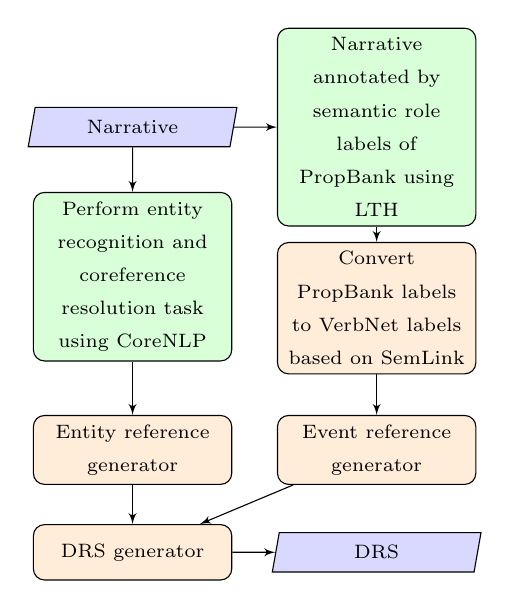
\begin{tikzpicture}[node distance=1.1cm, auto]
		\node (in1) [io] {\scriptsize Narrative};
		\node (pro1) [process1, right of=in1, xshift = 2cm,] {\scriptsize Narrative annotated by semantic role labels of PropBank using LTH};
		\node (pro2) [process1, below of=in1, yshift = -0.8cm] {\scriptsize Perform entity recognition and coreference resolution task using CoreNLP};
		\node (pro3) [process2, below of=pro1, yshift=-1.2cm] {\scriptsize Convert PropBank labels to VerbNet labels based on SemLink};
		\node (pro4) [process2, below of=pro2, yshift=-1.1cm] {\scriptsize Entity reference generator};
		\node (pro5) [process2, below of=pro3, yshift=-0.7cm] {\scriptsize Event reference generator};
		\node (pro6) [process2,below of=pro4, yshift=-0.2cm] {\scriptsize DRS generator};;
		\node (pro7) [io,right of=pro6, xshift=2cm] {\scriptsize DRS};
		
		\draw[arrow] (in1) -- (pro1);
		\draw[arrow] (in1) -- (pro2);
		\draw[arrow] (pro1) -- (pro3);
		\draw[arrow] (pro2) -- (pro4);
		\draw[arrow] (pro3) -- (pro5);
		\draw[arrow] (pro4) -- (pro6);
		\draw[arrow] (pro5) -- (pro6);
		\draw[arrow] (pro6) -- (pro7);
		
		\end{tikzpicture}
		\caption{System architecture}
    \end{wrapfigure}
    
    
	\noindent Figure 1 presents the Text2DRS's system architecture. The entity reference generator creates an entity coreference map from the CoreNLP output and uses this map to assign a reference ID to each distinct entity. From the LTH output, Text2DRS looks up the related VerbNet class information in the SemLink and returns the verb class number along with the respective thematic roles. However, sometime SemLink maps one PropBank predicate into multiple VerbNet classes. In this case, We pick the first verb class from the data list and use it in the final output. After entity reference generator and event reference generator complete process the data, the DRS generator merges the data and outputs the DRS for the given narrative.
	
    \subsection*{\small Future Work}
    \noindent Furthermore, SemLink doesn’t always contain the mapping of semantic role from the PropBank to the thematic role in the VerbNet. In some cases, we extended SemLink with missing mappings, and it is a future work effort to enhance SemLink further.

\begingroup
\setstretch{0.9}
\titleformat*{\section}{\normalfont}
\small{
\bibliography{Text2DRS}}
\endgroup

\end{document}